\section{Architettura}
L'architettura di \NomeProgetto{} è basata sul \glo{design pattern architetturale} \glo{\textit{Model-View-ViewModel (MVVM)}}, derivato dal più comune \glo{Model-View-Controller (MVC)}. 
Abbiamo quindi sviluppato un \textit{ViewModel} per ogni componente React della \textit{View} che necessita di interagire con il \textit{Model}, e delegato a tali \textit{ViewModel} la modifica del \textit{Model} in base agli input dell'utente. 
Il modello corrisponde al RootStore, che istanzia i tre diversi store utilizzati in \NomeProgetto{}. \\ \mbox{}\\
È stato scelto il design MVVM per i seguenti motivi: 
\begin{itemize}
	\item Favorisce la separazione tra \glo{\textit{business logic}} e \glo{\textit{presentation logic}}, facendo comunicare \textit{Model} e \textit{View} solo attraverso un \textit{ViewModel};  
	\item Permette di non avere un unico controller con cui dover gestire tutta l'\glo{\textit{application logic}}. Essa è infatti contenuta nei vari \textit{ViewModel} dei componenti della vista, fornendo diversi vantaggi: 
	\begin{itemize}
		\item Minor numero di conflitti in fase di codifica (non si deve accedere ad uno stesso file dove è contenuta tutta la logica);
		\item Performance migliori (viene renderizzato solo il componente che effettivamente subisce modifiche del proprio \glo{stato interno}, gestito anch'esso nel rispettivo \textit{ViewModel}).
	\end{itemize}
	\item Adatto per le web application la cui interfaccia utente è sviluppata con React.
\end{itemize}

\begin{figure}[hb]
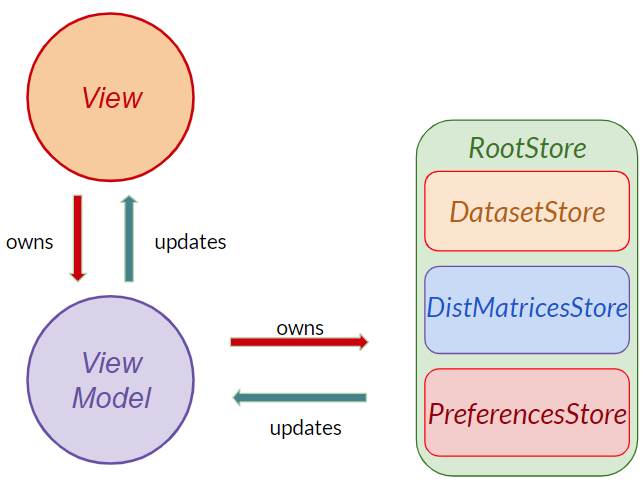
\includegraphics[width=11.8cm,height=8cm]{Extra/MVVMPattern}
\centering
\caption{Model-View-ViewModel di \textit{HDViz}}
\end{figure}

\newpage
\section{Diagrammi dei package}
\begin{figure}[hb]
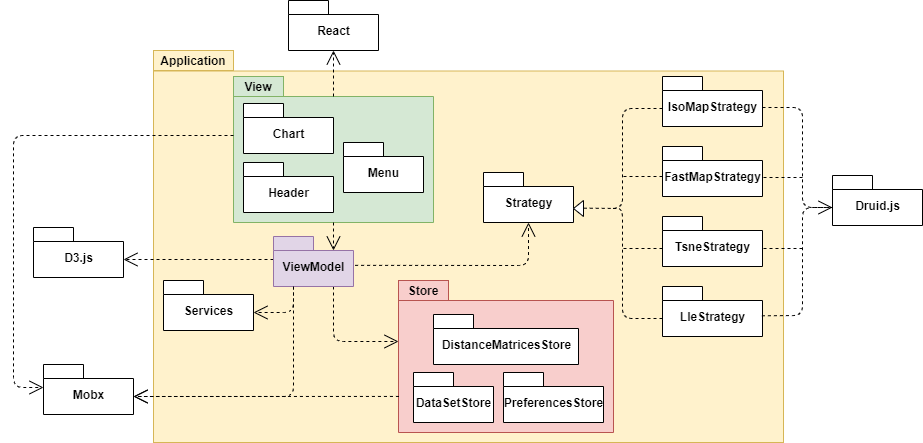
\includegraphics[width=15.8cm]{Images/Allegato Tecnico-Package}
\centering
\caption{Diagramma dei package client side}
\end{figure}

Il diagramma sopra riportato descrive a livello di package le parti che compongono il lato client dell'applicazione. In particolare si può notare come \textit{View} e \textit{Model} non siano direttamente collegati, ma il passaggio delle informazioni avviene attraverso il \textit{ViewModel} e il componente \glo{\textit{Context Provider}} fornito da React. \\ %componente fornito da React per consumare il contesto creato

\begin{figure}[hb]
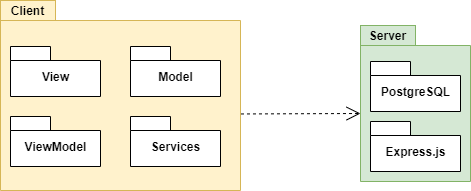
\includegraphics[width=15.8cm]{Images/Allegato Tecnico-Package 2}
\centering
\caption{Connessione tra client side e server side}
\end{figure}

\newpage
\section{Ciao}
\newpage
\subsection{Diagrammi di sequenza}
\begin{figure}[hb]
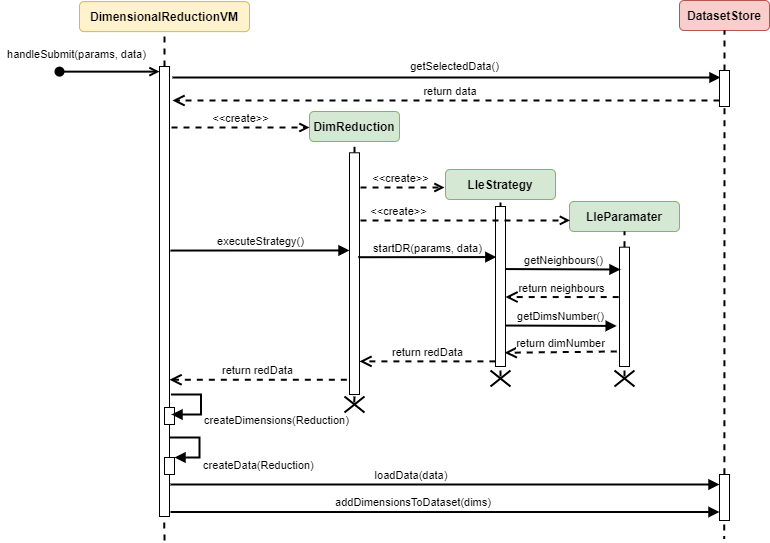
\includegraphics[width=16cm]{Images/Allegato Tecnico-Sequenza-DR}
\centering
\caption{Diagramma di sequenza che modella il processo di riduzione dimensionale con algoritmo LLE}
\end{figure}
Il diagramma di sequenza sopra riportato è cosi descritto:
\begin{enumerate}
	\item \textbf{DimensionalReductionVM}, che corrisponde al \textit{ViewModel} della parte di vista dedicata alla riduzione dimensionale, riceve l'algoritmo e i relativi valori dei parametri impostati dall'utente, prende i dati su cui eseguire la riduzione dal \textbf{DatasetStore} e crea il contesto, ossia \textbf{DimReduction};
	\item DimReduction si occupa di creare un'istanza della classe concreta dell'algoritmo scelto dall'utente (nell'esempio LLE, definito in \textbf{LLEStrategy}) e un'istanza della classe dei corrispettivi parametri (ossia \textbf{LLEParameter}), utilizzando i valori passatigli per settarne i vari attributi;
	\item Chiama poi \texttt{startDR()} sull'algoritmo, fornendo i dati e l'istanza della classe dei parametri. I valori di quest'ultimi vengono presi dall'algoritmo attraverso dei getter (nell'esempio \texttt{getNeighbours()} e \texttt{getDimensionsNumber()}) verso l'istanza di LLEParameter;
	\item \texttt{startDR()} a questo punto può eseguire la riduzione dimensionale utilizzando i metodi forniti dalla libreria Druid.js e ritornare un oggetto con dentro i nuovi dati e le nuove dimensioni;
	\item In DimensionalReductionVM vengono estrapolati i dati e le dimensioni dall'oggetto e caricate nel DatasetStore.
\end{enumerate}

\newpage
\begin{landscape}
\begin{figure}[hb]
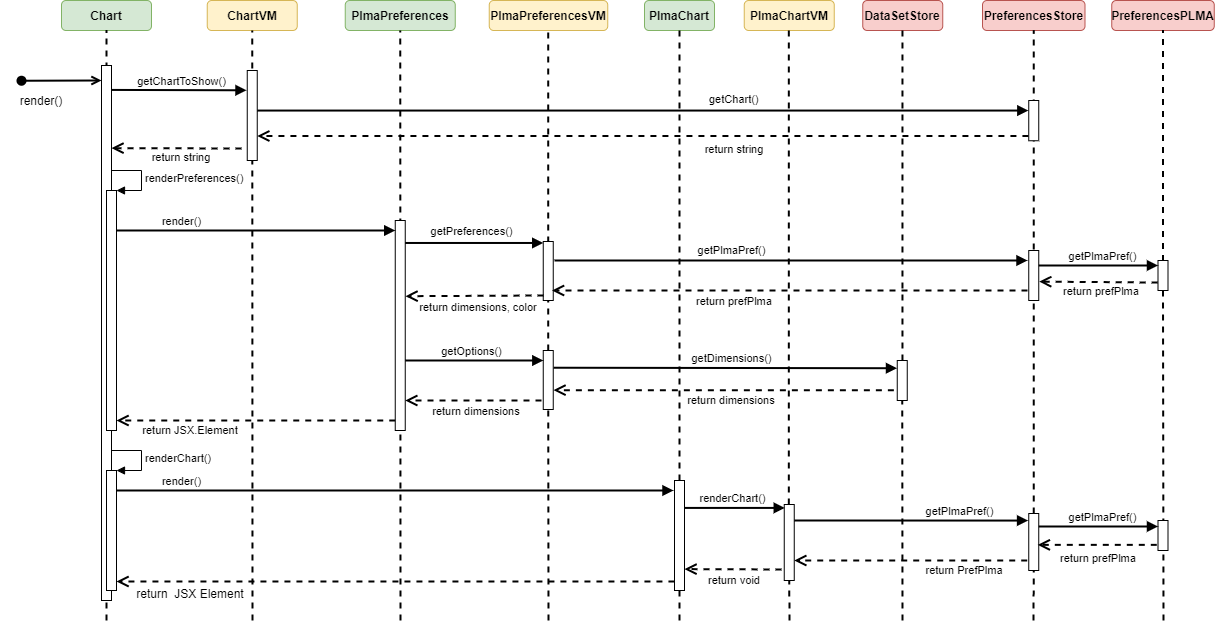
\includegraphics[width=\linewidth ,height=14cm]{Images/Allegato Tecnico-Sequenza-PLMApref}
\centering
\caption{Diagramma di sequenza che modella il processo di visualizzazione del grafico PLMA e del relativo box di preferenze}
\end{figure}
\end{landscape}
Il diagramma di sequenza sopra riportato è così descritto:
\begin{enumerate}[label=\textbf{\arabic*})]
	\item \textbf{Chart} è il componente React che renderizza la parte di vista contente il grafico e il relativo box di preferenze. Con \texttt{getChartToShow()} e \texttt{getChart()} di \textbf{ChartVM} (il corrispettivo \textit{ViewModel}) seleziona dal \textbf{PreferencesStore} la stringa che definisce quale box visualizzare (in questo esempio "PLMA");
	\item Sono quindi renderizzate le preferenze (\textbf{PlmaPreferences}), ossia la form utilizzabile dall'utente per modificare le caratteristiche di visualizzazione del PLMA. Inizialmente ogni suo campo input è vuoto e quindi non verrà visualizzato il grafico; 
	\item Ogni volta che l'utente modifica tale form avviene una rirenderizzazione del box delle preferenze e del grafico. Tale modifica comporta la chiamata al \textbf{PlmaPreferencesVM} (\textit{ViewModel} delle preferenze del PLMA) che si occupa di prelevare dai vari store (\textbf{PreferencesStore} e \textbf{DatasetStore}) le informazioni necessarie per cambiare in real-time la vista;
	\item È quindi renderizzato il PLMA (in \textbf{PLMAChart}) con le varie modifiche di visualizzazione impostate dall'utente.
\end{enumerate}

\newpage
\newpage
\subsection{Architettura di dettaglio: Strategy pattern} 
\begin{figure}[hb]
	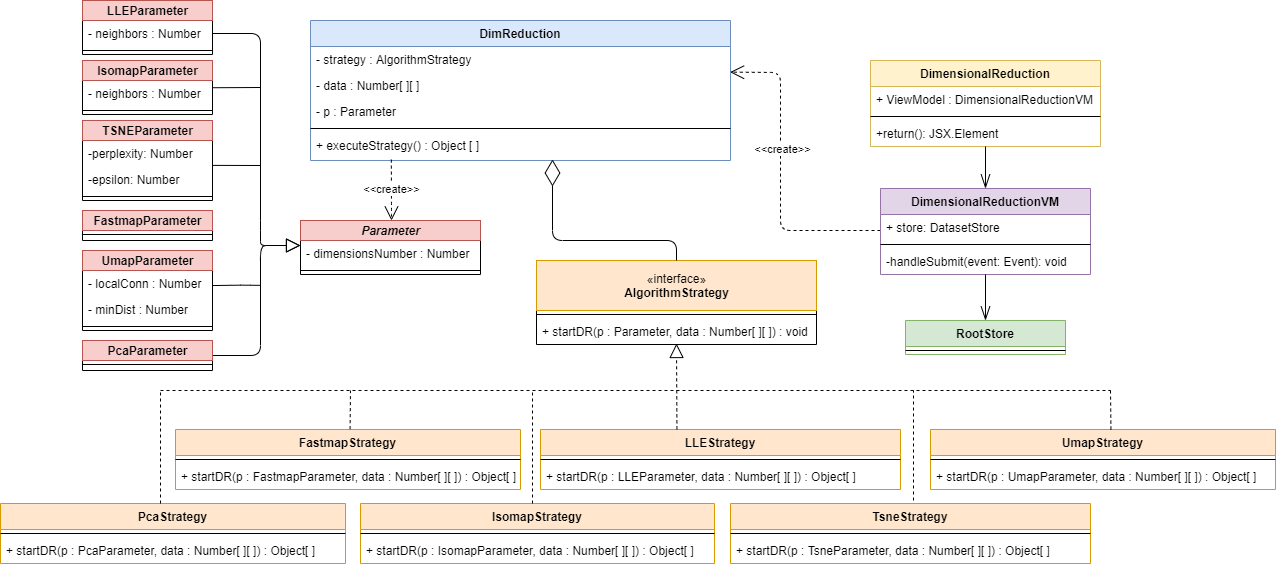
\includegraphics[width=17cm]{Images/StrategyPattern}
	\centering
	\caption{Strategy pattern per la scelta dell'algoritmo di riduzione dimensionale}
\end{figure}
Nella figura sopra è mostrata la funzionalità di riduzione dimensionale sui dati caricati dall'utente.
Per l'implementazione dei vari algoritmi viene utilizzato lo strategy pattern. In particolare:
\begin{itemize}
	\item \textbf{DimensionalReduction} è il componente React che si occupa solo di ritornare gli elementi HTML che compongono questa parte di vista;
	\item \textbf{DimensionalReductionVM} è il rispettivo view-model che ne contiene tutta la logica. Questo prende i dati dal RootStore (nello specifico dal \textit{DatasetStore}) e crea il contesto DimReduction;
	\item \textbf{DimReduction} si occupa di creare i parametri con i valori impostati dall'utente dalla vista. A seconda del valore del suo attributo \texttt{strategy} crea la corretta classe di parametri e chiama attraverso \texttt{executeStrategy()} il metodo \texttt{startDR()} sull'algoritmo scelto;
	\item \textbf{AlgorithmStrategy} è l'interfaccia implementata dalla famiglia di classi concrete degli algoritmi, facilitandone l'estensibilità.
\end{itemize} 

Infine \texttt{startDR()} esegue la riduzione dimensionale sui dati utilizzando i metodi forniti dalla libreria Druid.js e ritorna le nuove dimensioni.

